
\documentclass[tikz,border=6pt]{standalone}

\usepackage{amsmath}
\usepackage{tikz}

\usetikzlibrary{calc,angles,quotes}

\begin{document}
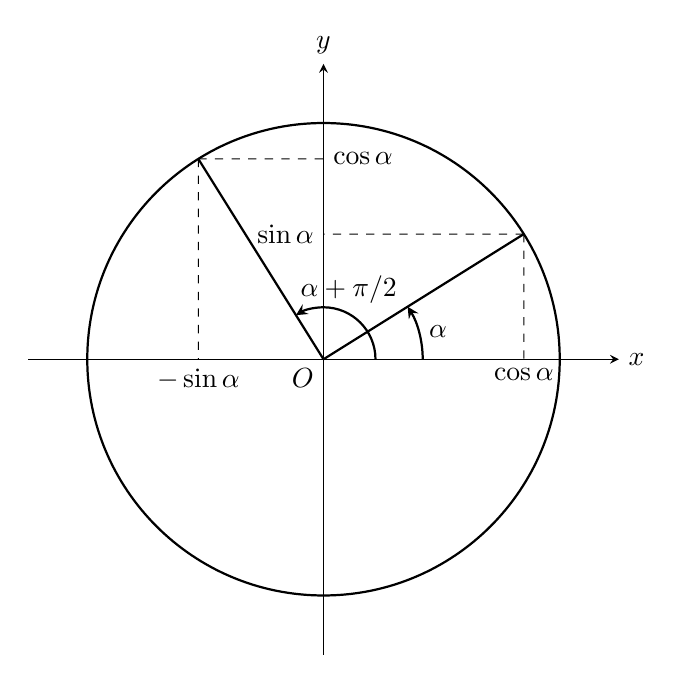
\begin{tikzpicture}[scale=3, >=stealth]

	\def\R{1}
	\def\ang{32} % angle in degrees

	\coordinate (O) at (0,0);

	\coordinate (P) at ({cos(\ang)},{sin(\ang)});
	\coordinate (Q) at ({-sin(\ang)},{cos(\ang)});

	\node[below left] at ($(O)$) {$O$};

	% axes
	\draw[->] (-1.25,0) -- (1.25,0) node[right] {$x$};
	\draw[->] (0,-1.25) -- (0,1.25) node[above] {$y$};

	% unit circle
	\draw[thick] (O) circle (\R);

	% radius to point P
	\draw[thick] (O) -- (P);

	% radius to point Q
	\draw[thick] (O) -- (Q);

	% projections
	\draw[dashed] (P) -- ({cos(\ang)},0)
	node[below] {$\cos\alpha$};
	\draw[dashed] (P) -- (0,{sin(\ang)})
	node[left] {$\sin\alpha$};

	\draw[dashed] (Q) -- ({-sin(\ang)},0)
	node[below] {$-\sin\alpha$};
	\draw[dashed] (Q) -- (0,{cos(\ang)})
	node[right] {$\cos\alpha$};

	% angle arc
	\draw[->, thick]
	(0.42,0) arc (0:\ang:0.42)
	node[midway, right] {$\alpha$};

	% angle arc
	\draw[->, thick]
	(0.22,0) arc (0:\ang+90:0.22)
	node[midway, above] {$\alpha+\pi/2$};

\end{tikzpicture}
\end{document}
